\chapter{Attachments} \label{chap:attachments}

% ~~~~~~~~~~~~~~~~~~~~~~~~~~~~~~~~~~~~~~~~~~~~~~~~~~~~~~~~~~~~~~~~~~~~~~~~~~~~~~~~~~~~~~~~~~~~~~~~~~~~~~~~~~~
\section{Algorithms, Functions, and Procedures} \label{sec:attachments/algorithms-functions-procedures}


\begin{alg}{Function}{GranularResourceLoad}{$k$, $\Instance$, $\Schedule$, $PC$} \label{alg:granular-resource-load}
\State $L : \intinterval{1}{PC} \to \Nzero$
       \Comment Period load function
\For {$j \in \JobsOnResource{k}$}
    \State $i_l \gets \lfloor \jobstart{j} / \algGranularity \rfloor$,
           \Comment{First overlapping period}
    \State $i_h \gets \lfloor \jobend{j} / \algGranularity \rfloor$
           \Comment{Last overlapping period}
    \If {$i_l = i_h$}
        \Comment{If the job overlaps with a single period...}
        \State $L(i_l) \gets L(i_l) + \duration{j} \consumption{j}{k}$
    \Else
        \Comment{...the job overlaps with multiple periods}
        \State $L(i_l) \gets L(i_l) + (\algGranularity (i_l + 1) - \jobstart{j}) \cdot \consumption{j}{k}$
        \For {$i \in \intinterval{i_l+1}{i_h-1}$}
            \State $L(i) \gets L(i) + \algGranularity \cdot \consumption{j}{k}$
        \EndFor
        \State $L(i_h) \gets L(i_h) + (\jobend{j} - \algGranularity (i_h - 1)) \cdot c$
    \EndIf
\EndFor
\State \Return $L$
\end{alg}


\begin{alg}{Function}{IncreaseGranularPeriodCapacity}{$i$, $\capacityf{k}$, $\algGranularity$, $\algImprovement$} \label{alg:increase-granular-period-capacity}
\State $t_l \gets 1+ (i-1)\algGranularity$
       \Comment First time period covered
\State $t_h \gets i \algGranularity$
       \Comment Last time period covered
\For{$t \in \intinterval{t_l}{t_h}$}
    \State $\capacity{k}{t} \gets \capacity{k}{t} + \algImprovement$
\EndFor
\State \Return $\capacity{k}{t}$
\end{alg}


\begin{alg}{Function}{ReduceCapacityChanges}{$\Instance$, $\Schedule$, $\capacityf{1}^\text{orig}$, \dots, $\capacityf{m}^\text{orig}$} \label{alg:reduce-capacity-changes}
\State $\capacityf{1}^\prime, \dots, \capacityf{m}^\prime: \intinterval{1}{\horizon} \to \Nzero$
       \Comment Reduced capacity functions
\For {$k \in \Resources$}
    \State $L \gets $ \Callref{ResourceLoad}{$k$, $\Instance$, $\Schedule$}{alg:resource-load}
    \For {$t \in \intinterval{1}{\horizon}$}
        \State $\capacity{k}{t}^\prime \gets \max(\capacity{k}{t}^{\text{orig}}, L(t))$
    \EndFor
\EndFor
\State \Return $\capacityf{1}^\prime, \dots, \capacityf{m}^\prime$
\end{alg}


\begin{alg}{Function}{ResourceLoad}{$k$, $\Instance$, $\Schedule$} \label{alg:resource-load}
\State $L : \intinterval{1}{\horizon} \to \Nzero$
\For {$t \in \intinterval{1}{\horizon}$}
    \State $L(t) \gets \sum_{j \in \JobsOnResourceInTimePeriod{k}{t}} \consumption{j}{k}$
        \Comment $\JobsOnResourceInTimePeriod{k}{t}$ with respect to given schedule $\Schedule$
\EndFor
\State \Return $L$
\end{alg}


\begin{alg}{Function}{FindAdditionsAndMigrations}{$\Instance$, $\Schedule$} \label{alg:find-additions-and-migrations}
\State $\Migrations \gets \emptyset$
\For {$(\forall k \in \Resources)$} $L_k \gets$ \Callref{ResourceLoad}{$k$, $\Instance$, $\Schedule$}{alg:resource-load} \EndFor
\For {$(\forall k \in \Resources)$} $\capacityf{k}^\oplus \gets \capacityf{k} - L_k$ \Comment Capacity surpluses \EndFor
\State REQ $\gets$ set of all additional non-shift capacities

\For {$(k, s, e, c) \in$ REQ}
    \While {$c > 0$}
        \State $c_1, \dots, c_m \gets$ maximal continuous surpluses overlapping $\intinterval{s}{e}$
        \State $k_\text{from} \gets \argmax_k{c_k}$
        \If {$c_{k_\text{from}} = 0$} \Comment If no further migrations are possible
            \State \textbf{break} \Comment Remaining $c$ will be fulfilled by capacity additions
        \EndIf
        \State $c_\text{mig} \gets \min(c, c_{k_\text{from}})$
        \State Reduce surplus $\capacityf{k_{\text{from}}}^\oplus$ by $c_{\text{mig}}$ during time periods $\intinterval{s}{e-1}$
        \State $\Migrations \gets \Migrations \cup \{ \migration{k_\text{from}}{k}{s}{e}{c_{\text{mig}}} \}$
    \EndWhile
\EndFor

\State $\Additions \gets \left\{ \addition{k}{s}{e}{c} \in \text{ REQ} : c > 0 \right\}$

\State \Return $\Additions$, $\Migrations$
\end{alg}


\begin{alg}{Function}{ModifyResourceCapacities}{$\Instance$, $\chi_1$, \dots, $\chi_c$} \label{alg:modify-resource-capacities}
\State $\capacityf{1}^*, \dots, \capacityf{m}^* \gets \capacityf{1}, \dots, \capacityf{m}$
    \Comment Copy the original capacity functions
\For {$(j, s, e) \in \{ \chi_1, \dots, \chi_c \}$}
    \For {$k \in \Resources : \consumption{j}{k} > 0 $}
        \For {$t \in \intinterval{s}{e-1}$}
            \State $\capacity{k}{t}^* \gets \capacity{k}{t}^* + \consumption{j}{k}$
        \EndFor
    \EndFor
\EndFor
\State \Return $\capacityf{1}^*, \ldots, \capacityf{m}^*$
\end{alg}


\begin{alg}{Function}{ComputeSuffixRelaxedSchedule}{$\Instance$, $\Schedule$, $t$} \label{alg:suffix-relaxed-schedule}
\State $T \gets $ Topological ordering of $\Jobs$ on the precedence graph $G$
\For {$j \in T$}
    \If {$\jobstart{j} \leq t$}
        \State $\relaxedjobstart{t}{j} \gets \jobstart{j}$
    \Else
        \State $\relaxedjobstart{t}{j} \gets \max\left\{\relaxedjobstart{t}{i} + \duration{i} : \precedence{i}{j} \in \Precedences \right\}$
    \EndIf
\EndFor
\State \Return $\relaxedSchedule{t}$
\end{alg}

\newpage
\begin{alg}{Function}{ComputeLeftShiftClosure}{$\Instance$, $\Schedule$, $j$} \label{alg:left-shift-closure}
\State $\closure{j} \gets \emptyset$
\State $Q \gets \{j\}$ \Comment Queue of jobs to process
\While {$Q \text{ not empty}$}
    \State $i \gets$ pop $Q$
    \State $\closure{j} \gets \closure{j} \cup \{ i \}$
    \State $Q \gets Q \cup \{ p : \precedence{p}{i}, \jobend{p} = \jobstart{i}\}$
        \Comment Precedence predecessors
    \State $Q \gets Q \cup \bigcup_{k: \consumption{i}{k} > 0}\{ p \in \JobsOnResource{k} : \jobend{p} = \jobstart{i} \}$
        \Comment Resource predecessors
    \For {$k \in \Resources, \consumption{i}{k} > 0, \capacity{k}{\jobstart{i}-1} = 0$}
        \Comment Resource-pause predecessors
        \State $\mathrm{ps}_k(\jobstart{i}) \gets \max\{t^\prime \in \intinterval{1}{\jobstart{i}-1} : \capacity{k}{t^\prime} > 0\}$
        \State $Q \gets Q \cup \{ p \in \JobsOnResource{k} : \mathrm{ps}_k(\jobstart{i}) - \duration{i} \leq \jobend{p} \leq \mathrm{ps}_k(\jobstart{i}) \}$
    \EndFor
\EndWhile
\State \Return $\closure{j}$
\Statex
\Note  We assume, that when the value of $\mathrm{ps}_k(\jobstart{i})$ is undefined,
       the following set of predecessors
\Notec is trivially empty and we continue with a different resource.
\end{alg}

% ~~~~~~~~~~~~~~~~~~~~~~~~~~~~~~~~~~~~~~~~~~~~~~~~~~~~~~~~~~~~~~~~~~~~~~~~~~~~~~~~~~~~~~~~~~~~~~~~~~~~~~~~~~~
\section{Documentation} \label{sec:attachments/documentation}

This section contains the description of the project implementing the algorithms and running the experiments
presented in this thesis.
The full project is attached in the \texttt{RCPSPSandbox.zip} file.
The repository of the project can be found online at \url{https://github.com/Krtiiik/RCPSPSandbox}.

% -----------------------------------------------------------------------------------------------------------
\subsection{Requirements}

All implementations are written in Python, utilizing several external libraries.
To run scripts, the following is required:

\begin{itemize}
    \item Python 3.11 with installed packages listed in the \texttt{requirements.txt} file.

    \item Configured IBM ILOG Constraint-Programming Optimizer.
        IBM ILOG Constraint-Programming Optimizer is part of the IBM ILOG CPLEX Optimization Studio
        commercial software package.
        Community and academic editions are available.
        See online at \url{https://www.ibm.com/products/ilog-cplex-optimization-studio/cplex-cp-optimizer}.
\end{itemize}

Python version at least 3.11 is required as we utilize several functionalities introduced in that version.
However, note that the \texttt{docplex} library does not fully support this version.
We had no issues with this partial incompatibility.

% -----------------------------------------------------------------------------------------------------------
\subsection{Running scripts}

A simple example demonstrating the two algorithms presented in this thesis
is contained in the \texttt{rcpsp\_sandbox/example.py} script file.
Input and resulting data of this example is located in the \texttt{example} directory.

All experiments are run using the \texttt{experiments.py} Python script file,
located in the \texttt{rcpsp\_sandbox} source directory.
Following is the invocation help:

\begin{small}
\begin{verbatim}
usage: experiments.py [-h] [--save_plots] [--addition ADDITION]
                      [--migration MIGRATION]

options:
  -h, --help             show this help message and exit
  --save_plots           Determines whether to save plots to files
  --addition ADDITION    Cost of capacity addition (default is 5)
  --migration MIGRATION  Cost of capacity migration (default is 1)
\end{verbatim}
\end{small}

Running this script computes the experiments.
The script evaluates the algorithms (or loads computed evaluations from data files),
computes statistics, which are then saved to data files,
and finally creates plots of the results.

We provide the computed results in the \texttt{data} directory.
In this directory, base instances, modified instances,
and computed evaluations and evaluation KPIs are stored
in directories named accordingly.
Before running the experiments, the \texttt{modified\_instances} directory has to be extracted
from a zip file named \texttt{modified\_instances.zip}.

% -----------------------------------------------------------------------------------------------------------
\subsection{Project overview}

The project is divided into the following sub-packages, each containing several modules:

\begin{itemize}
    \item \texttt{rcpsp\_sandbox.instances} --- modules for manipulating problem instances.
    \item \texttt{rcpsp\_sandbox.solver} --- modules for solving the problem instances.
    \item \texttt{rcpsp\_sandbox.bottlenecks} --- modules implementing the presented algorithms
        and hosting experiment evaluations.
\end{itemize}

The \texttt{rcpsp\_sandbox.instances} sub-package contains several modules for manipulating with problem instances.
Those modules are used in the rest of the project, forming a core data infrastructure.
In the \texttt{problem\_instance} module contains the definition of the \texttt{ProblemInstance}
class, representing the problem instance defined in \cref{def:problem-instance}.
The \texttt{io} module is used for parsing and serializing problem instance object,
be it in the original PSPLIB file format, or in JSON.
The \texttt{problem\_modified} module provides the \texttt{modify\_instance} function,
which for a given problem instance returns a \texttt{ProblemModifier} object.
The interface of the object allows the user to modify all aspects of the problem instance.
Most important, it implements the modifications described in \cref{sec:problem-statement/scheduling},
namely, splitting the precedence graph, introducing time-variable resource capacities,
assigning job due dates.
The \texttt{algorithms} module implements several algorithms regarding problem instances,
mostly various precedence graph traversals.

The \texttt{rcpsp\_sandbox.solver} sub-package contains, among others, the \texttt{solver} module.
This module facilitates the solving of problem instances via the \texttt{Solver} class.
The \texttt{Solver} class contains a single \texttt{solve} method, which takes in either a problem instance,
of a built model to solve.
The function utilizes the \texttt{docplex} library to call the IBM ILOG Constraint-Programming Optimizer
solver, which finds (optimal) solutions to given models.
If a problem instance is given to the \texttt{Solver.solve} method,
the solver builds a standard model described in \cref{sec:problem-statement/constraint-programming-model}.
For a finer control over the model, the \texttt{model\_builder} module provides the \texttt{build\_model} function.
This function, for a given problem instance, return an initialized \texttt{ModelBuilder} object.
The interface of this object allows for the creation of specific models,
introducing only selected constraints, restraining job intervals, or choosing alternate optimization goals.
The \texttt{solution} module contains the definition of the \texttt{Solution} abstract class,
along with several implementing derived classes and utility functions concerning solutions to the problem instance models.

The \texttt{rcpsp\_sandbox.bottlenecks} sub-package contains the implementations of the \acl{iira} and \acl{ssira},
and a framework for evaluating the algorithms on problem instances.
The \texttt{improvements} module contains the algorithms' implementations
together with implementations of helper functions from \cref{sec:attachments/algorithms-functions-procedures}.
The \texttt{evaluations} module contains the \texttt{evaluate\_algorithms} and the \texttt{compute\_evaluation\_kpis} functions.
Those are central for the experiments: the former runs the algorithms with specified parameters on a given problem instance
and return the sets of computed evaluations, the latter computes the experiment KPIs of the evaluations.

Following is a minimal working example of evaluating both algorithms utilizing the \texttt{evaluate\_algorithms} function
on a problem instance parsed from the \texttt{instance.json} file.
The set of all algorithm parameters is the exact same set used for the experiments conducted in \cref{chap:numerical-experiments}.

\begin{python}
import rcpsp_sandbox.instances.io as iio
from rcpsp_sandbox.bottlenecks.evaluations \
    import evaluate_algorithms

instance = iio.parse_json("instance.json", is_extended=True)
evaluations = evaluate_algorithms(instance, [
    (ScheduleSuffixIntervalRelaxingAlgorithm(), {
        "max_iterations": [1, 2, 3],
        "relax_granularity": [1],
        "max_improvement_intervals": [1, 2, 3, 4, 5, 6],
        "interval_sort": ["improvement", "time"]}),
    (IdentificationIndicatorRelaxingAlgorithm(), {
        "metric": ["auau", "mrur"],
        "granularity": [4, 8],
        "convolution_mask": ["pre1", "around", "post"],
        "max_iterations": [1, 2, 3],
        "max_improvement_intervals": [1, 2, 3, 4],
        "capacity_addition": [4, 10]}),
])
\end{python}

The \texttt{rcpsp\_sandbox.manager} module contains the \texttt{ExperimentManager} class,
which manages loading and saving of experiment evaluations, KPIs, and problem instances.
It can be passed to the \texttt{evaluate\_algorithms} function
to attempt loading existing evaluations from files before computing them anew.

% ~~~~~~~~~~~~~~~~~~~~~~~~~~~~~~~~~~~~~~~~~~~~~~~~~~~~~~~~~~~~~~~~~~~~~~~~~~~~~~~~~~~~~~~~~~~~~~~~~~~~~~~~~~~
\section{Full instance plots} \label{sec:attachments/full-instance-plots}

\begin{figure}[p]
    \centering
    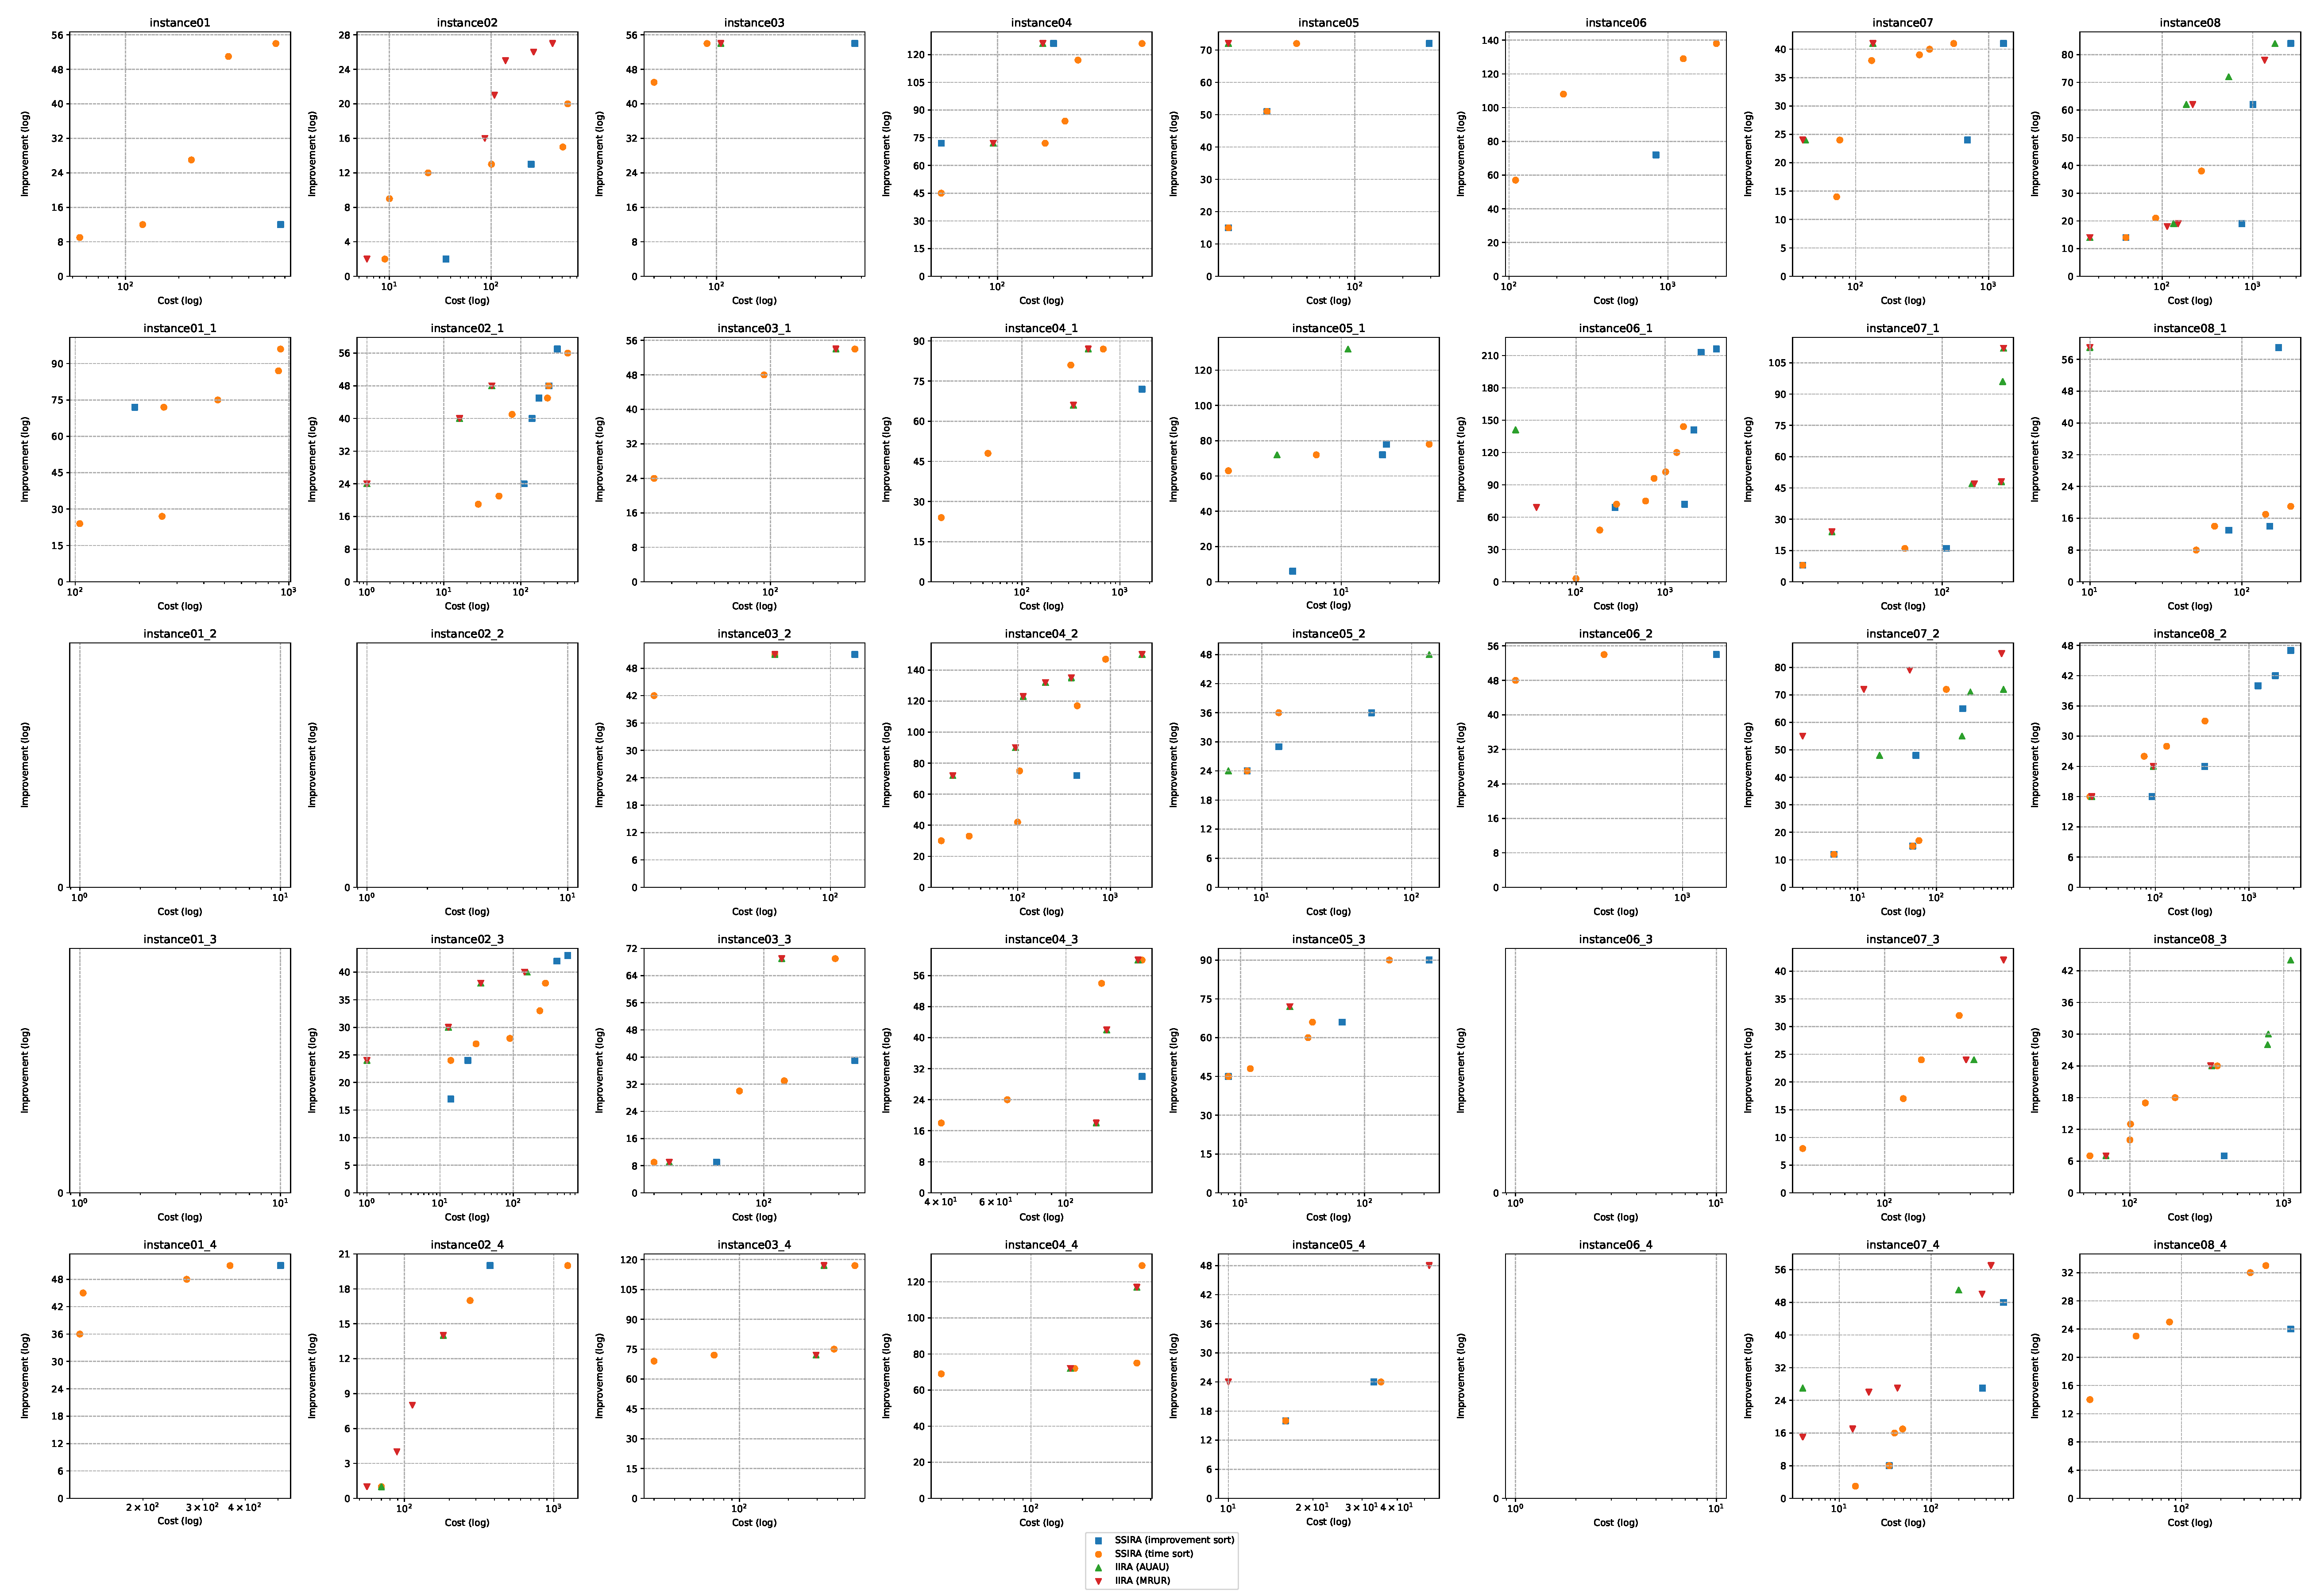
\includegraphics[angle=270, width=\textwidth]{img/exp_cost_improv.pdf}
    \caption{
        Capacity changes cost (x-axis) to achieved 
        improvement (y-axis) for every experiment instance.
        }
    \label{fig:exp-full/cost-improv}
\end{figure}

\begin{figure}[p]
    \centering
    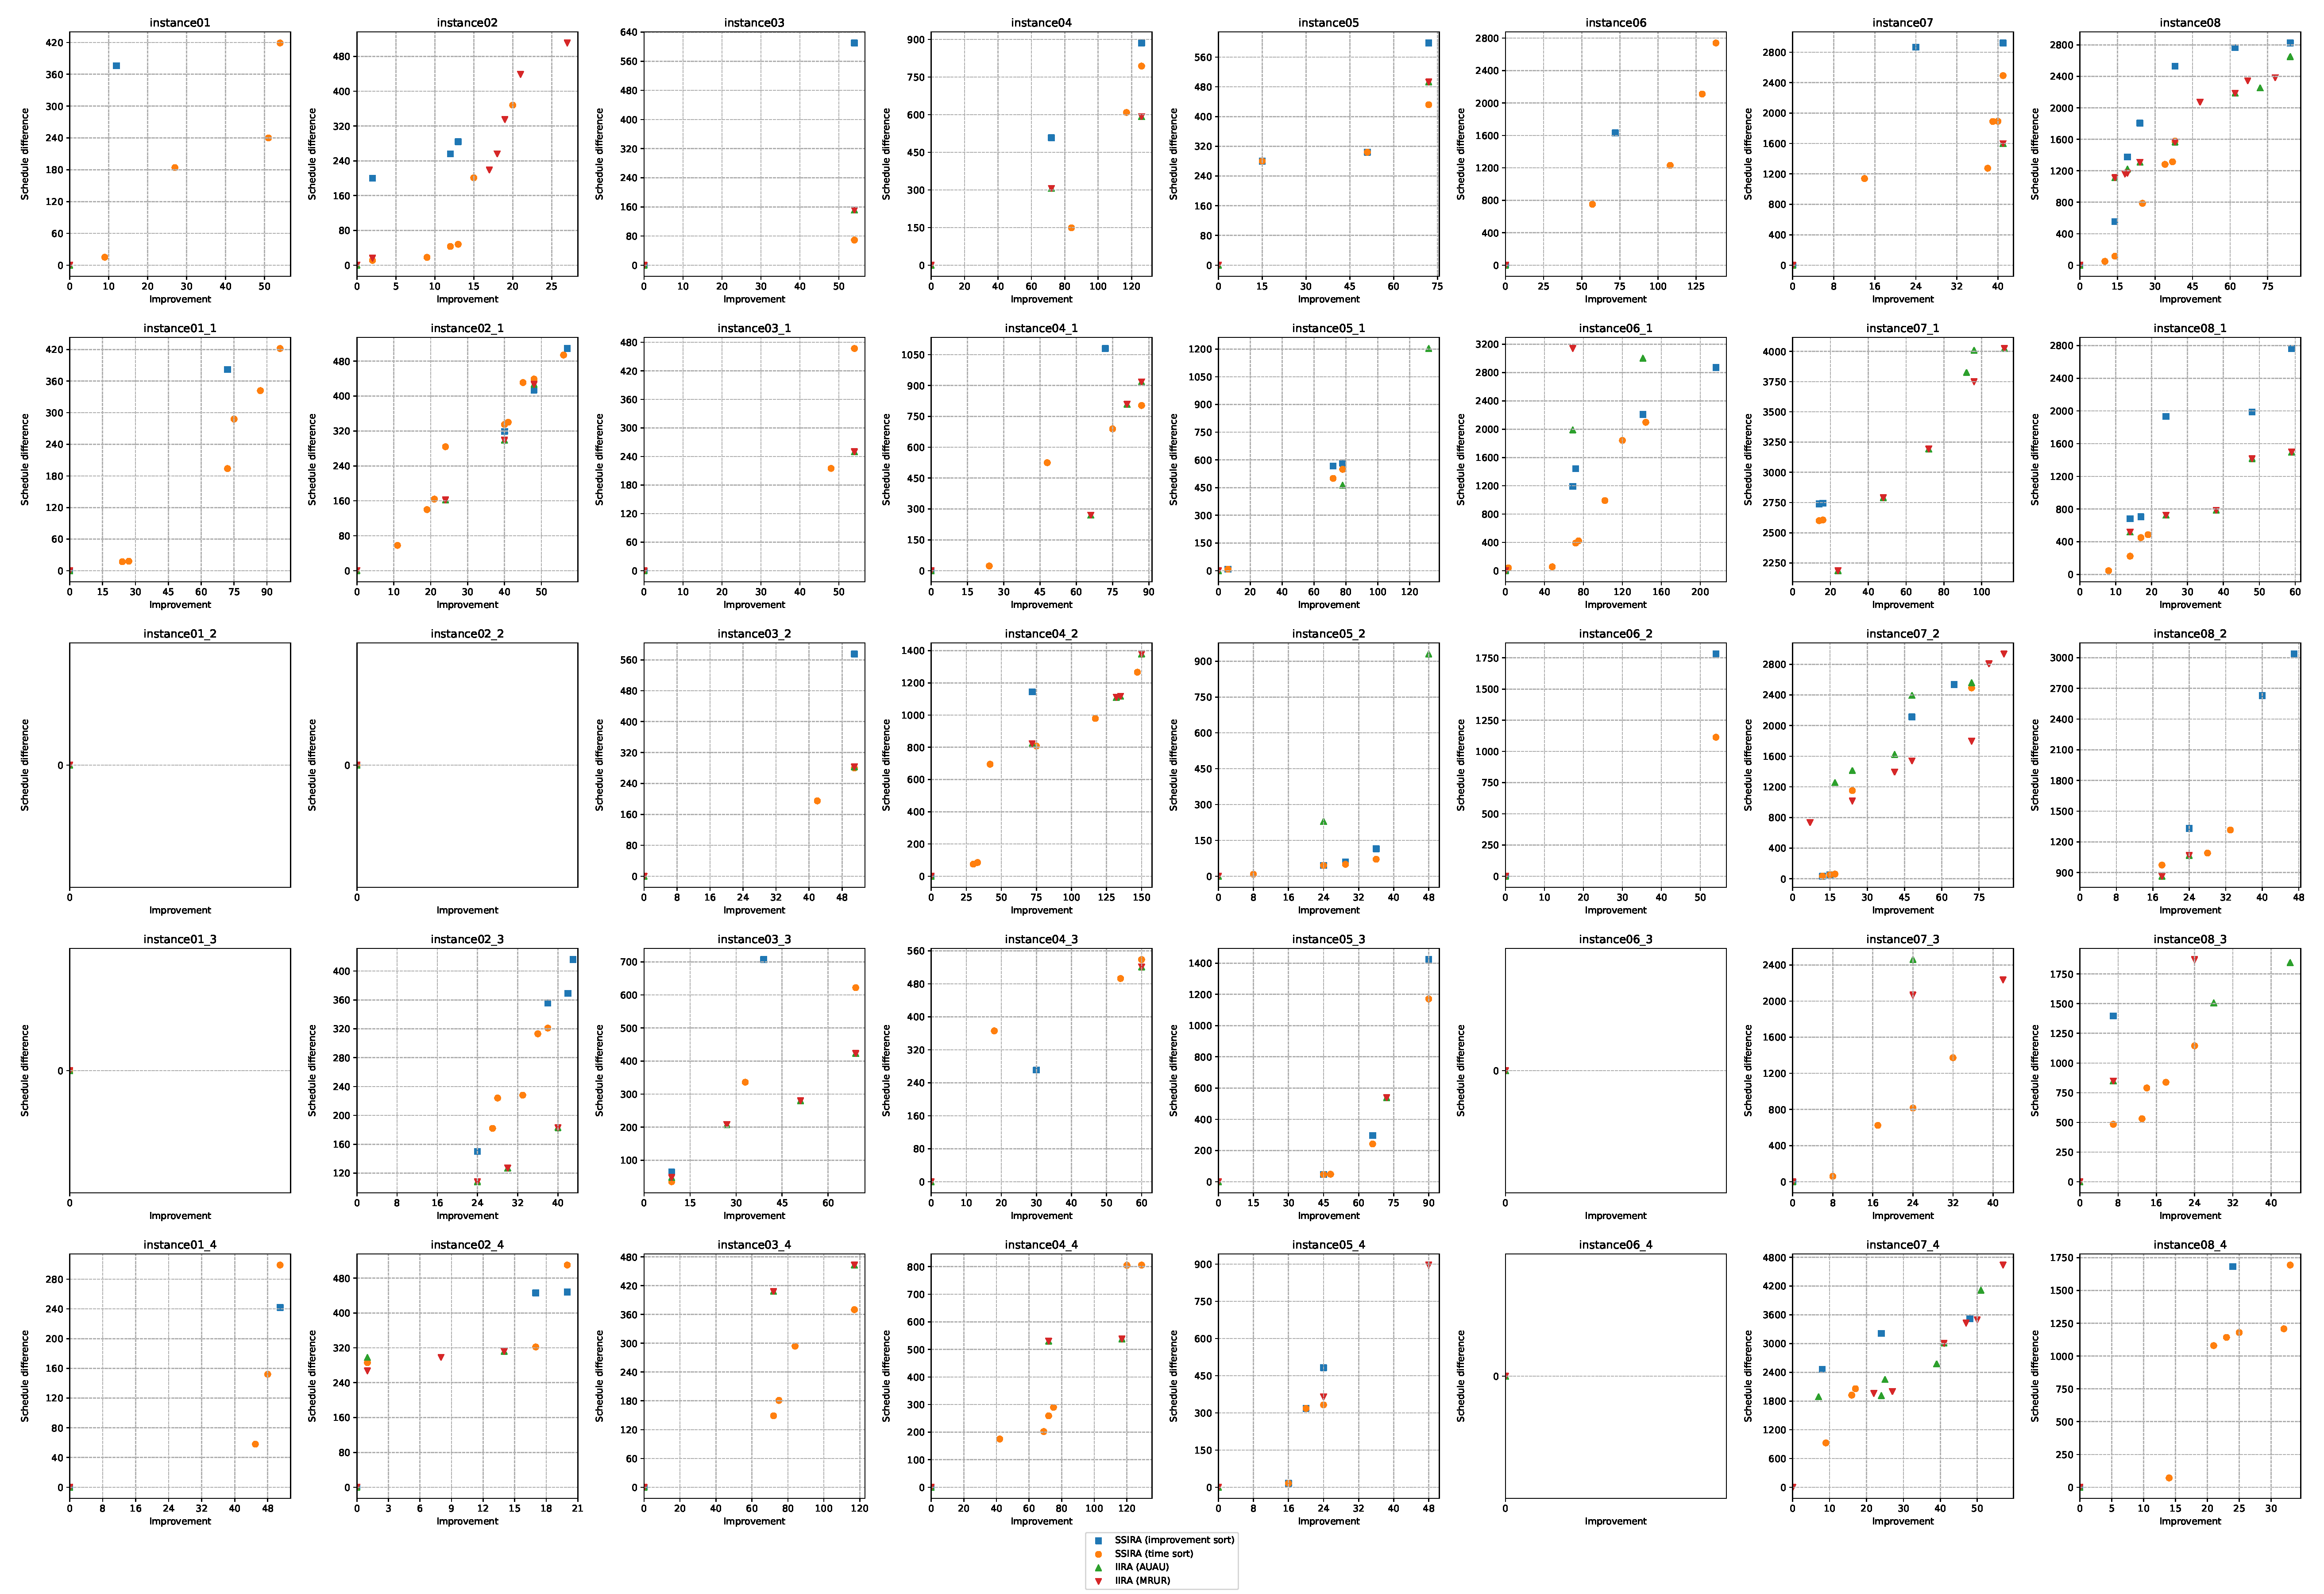
\includegraphics[angle=90,width=\textwidth]{img/exp_improv_diff.pdf}
    \caption{
        Achieved improvement (x-axis) to schedule
        difference (y-axis) for every experiment instance.
        }
    \label{fig:exp-full/improv-diff}
\end{figure}

\begin{figure}[p]
    \centering
    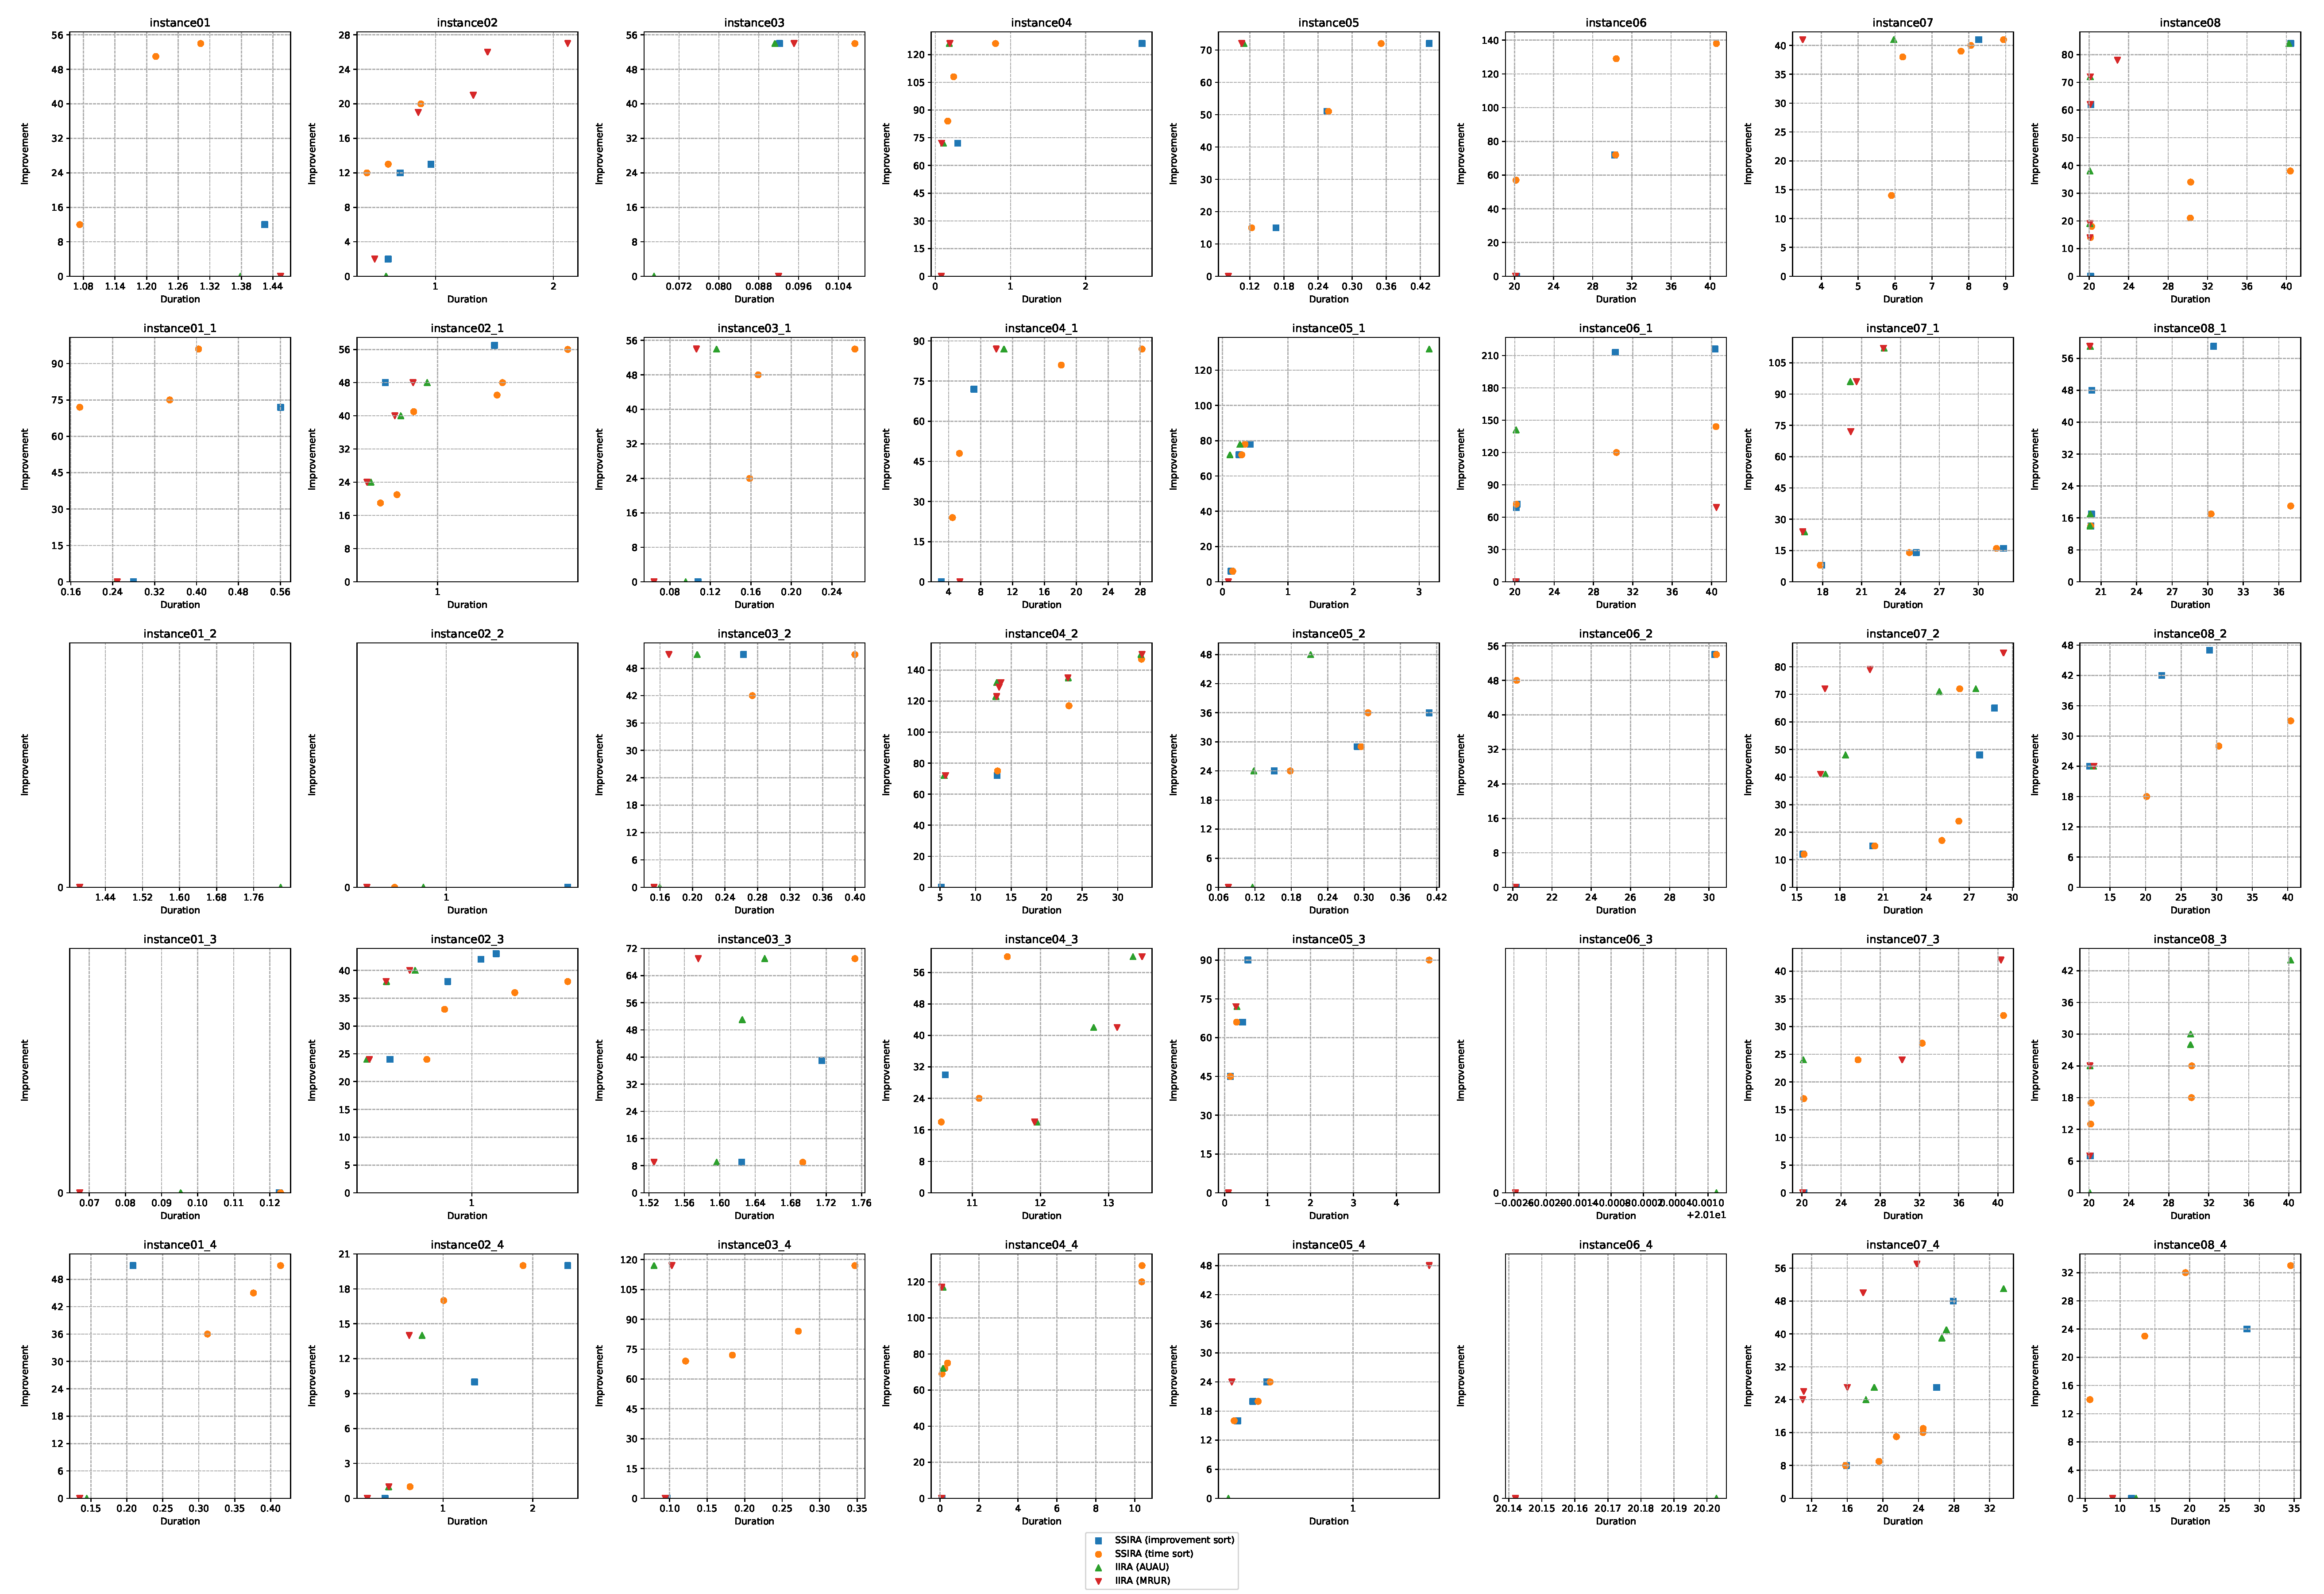
\includegraphics[angle=270,width=\textwidth]{img/exp_duration_improv.pdf}
    \caption{
        Evaluation duration (x-axis) to achieved
        improvement (y-axis) for every experiment instance.
        }
    \label{fig:exp-full/duration-improv}
\end{figure}
